\newpage
\section{The Experiment}
\label{experiment}

The goal of this section is to explain the experiment with all technical detail needed, from adopted models to results through scenarios and measures.\\
First of all experiment aims to measure efficiency of several forwarding algorithm in an infrastructure free scenario, where mobile nodes are able to interact with others only in a limited local area around them. \\
We measure forwarding algorithm performance in terms of:
\begin{list}{}
\item \emph{Delivery ratio}: $ \dfrac{Number Of Messages Delivered}{ Number Of Messages Sent } $ 
\item \emph{Delivery cost}:  $ \dfrac{Number Of Inflight Messages }{ Number Of Messages Sent } $
\end{list}
Delivery ratio could range from $0$ to $1$, and we are interested in the maximum delivery ratio value obtained through all simulation time. We care about maximum value in the all time span because we are simulating an opportunistic delay tolerant network. For delivery cost we consider it's maximum value (cost peek), it's average value and it's variance across the simulation time, and its correlation with delivery ratio.\\ 

\subsection{Models and algorithms}
\label{exp_incarnation}
Since experiment needs to simulate a realistic contact network dynamics, we based our simulation on the community based mobility model introduced in section\ref{mobility_community_based_model} which is able to reproduce credible human-like interaction traces. In order to use this tool we had to generate a social-network to feed the mobility model algorithm.\\
For this reason we choose to adopt the caveman enhanced network model described in section\ref{sn_caveman_model} where community structures are first class concept.\\
Also we implement a subset of the forwarding algorithm described in\ref{forwarding}, both social-based and non-social ones; in detail we ran experiment with the following forwarding algorithms:
\begin{itemize}
\item \emph{Flood}, which is the most effective algorithm (but also the most expensive in terms of message copies)
\item \emph{Label}, which exploit node's interests and consequential community patterns.
\item \emph{Rank}, where nodes popularity lead forwarding decisions.
\item \emph{Bubble}, where both node's interest and popularity are exploited according to algorithm\ref{r_bubble_alg}.
\end{itemize}

\subsection{Simulation platform}
\label{exp_platform}

We decide to use a simulation platform that lessen the abstraction gap between the conceptual space of our experiment and the platform abstractions. In detail our experiment mainly involves two main concepts: mobile nodes and social networks.\\
Since we think supporting mobility simulation is generally harder than supporting social network simulations we choose to adopt the \emph{Alchemist} simulation platform\cite{pianini-jos2013} because it has been explicitly designed to handle nodes mobility and contact networks.\\
A part of the class project work has been allocated in the extension of the Alchemist platform in order to: 
\begin{itemize}
\item Integrate the concept of social network and enable simulation on arbitrary topologies.
\item Design a mechanism which permit to define arbitrary network formation algorithm (aka auto-linking rule)\footnote{Alchemist use an auto-linking euclidean rule (based on euclidean distance) for determining when a mobile node has a neighbourhood relationship with another one}.
\item Support environment with multiple networking layers. For instance support an euclidean environment with mobile nodes that links each others based on their physical distance, and at the same time support the concept social neighbourhood, or in general another linking layer based on other - non euclidean - criteria.
\end{itemize}

With this extensions we are fully enabled to run the experiment described above, which exploits only a small part of the expressive power of this extension.\\
In fact adding a social networking conceptual space to alchemist's domain may enable simulations on social network formation and dynamics by simulating contacts and interactions between mobile nodes in several environmental conditions.\\

\subsubsection{Experiment set-up}
\label{exp_setup}

In order to obtain a significant statistical base we set-up 2 experimental session:
\begin{itemize}
\item First one composed by 100 runs for each forwarding algorithm with 60 mobile nodes\footnote{Datasets used for emulations in\cite{bubble} provide traces of a number of mobile devices between 40 and 100 units} distributed in 6 communities and 16 message to deliver (uniformly distributed across nodes population), each time with a randomized\footnote{We used the built-in Mersenne Twister algorithm provided by simulation platform} initial configuration in terms of relationship between mobile users and consequential contact traces.
\item Second one with the same characteristics of the previous except for the number of message to deliver: 100 per run. 
\end{itemize}
In these experiments we set-up all messages at configuration time, so every sender start delivering from the beginning of the simulation. This configuration make sense if we assume that the stochastic process we are simulating is ergodic, under this assumption we might consider the simulation as a valid time sample of the behaviour of the system under the specified load (in terms of message to deliver in a time span).\\
In figure \ref{fig:bubble_live_init} and \ref{fig:bubble_live} are represented environment and nodes in the simulation demo running on Alchemist.
\begin{figure}[h!]
	\begin{center}
    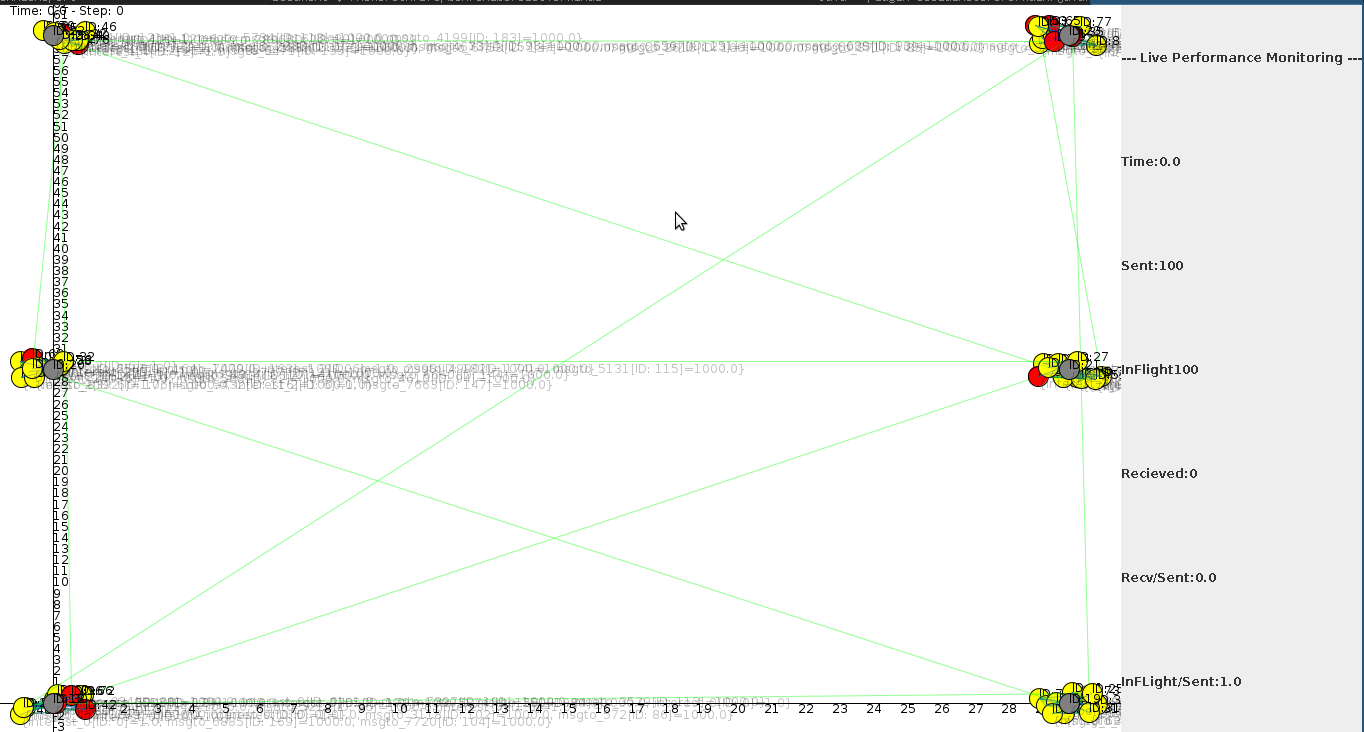
\includegraphics[scale=0.25]{img/bubble_live_init.png}
    \caption{Simulation initial configuration. Green lines represent social relationship while blue (shorter) lines physical links.}
    \label{fig:bubble_live_init}
  \end{center}
\end{figure}
\begin{figure}[h!]
	\begin{center}
    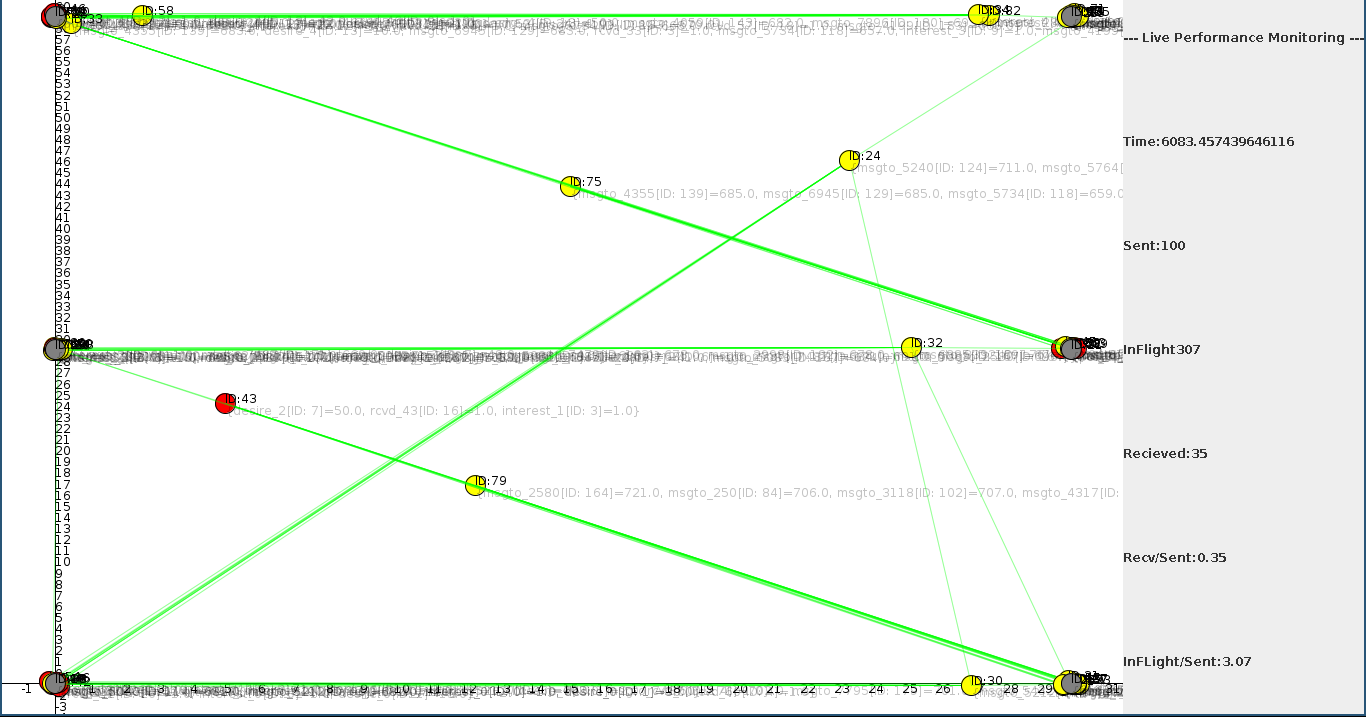
\includegraphics[scale=0.25]{img/bubble_live.png}
    \caption{Running simulation (bubble)}
    \label{fig:bubble_live}
  \end{center}
\end{figure}

\newpage
\subsubsection{Original Experiment}
In honour of completeness we briefly report emulation parameters and measurements reported in\cite[Table 3,6.2]{bubble}. The reference experiment - based on \emph{Reality data set} - involves 73 nodes subdivided in 8 communities (average size $\sim 9$) and a simulation time of 3 weeks. In figure \ref{fig:reality_emulation} are shown delivery ratio and cost measured during simulations.
\begin{center}
\begin{figure}[h!]
    		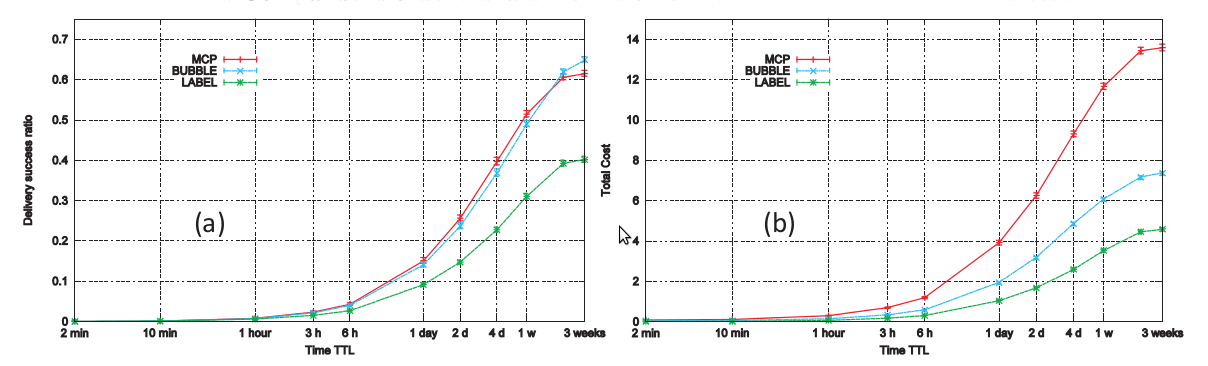
\includegraphics[scale=0.35]{img/reality_emulation.png}
    		\caption{Comparison of several algorithm performance reported in \cite{bubble} with \emph{Reality data set}. Figures \emph{a} and \emph{b} shows delivery ratio and cost respectively}
    		\label{fig:reality_emulation}
\end{figure}
\end{center}

\newpage
\subsection{Results}
\label{exp_results}

Simulation results have shown similar motifs with respect to emulation performed in\cite{bubble} and reported in figure\ref{fig:reality_emulation}, but values does not perfectly fit each others in term of absolute values. In fact we might note social based algorithm have lower delivery cost with respect to classical ones (eg. MCP in fig.\ref{fig:reality_emulation} and Flood in our experiments, fig.\ref{fig:run_1_aggregate}) and bubble algorithm has higher delivery ratio with respect to other social based algorithms.\\
The value difference could be caused by the load assumptions performed and the time span considered.\\
In fact in\cite[6.2]{bubble} time span considered is 3 week large ($1814400 sec$), with a presumable node velocity of $1\sim1.5 \frac{m}{sec^{-1}}$, instead simulated experiments range within 7 hours ($\sim 25000 sec$). So the 1000 message of the emulation are spread in a larger time span, with an average ratio of $5.5\cdot 10^{-4}$, while the 100 messages of the simulation are cumulated in a smaller time interval, with average ratio of $4\cdot 10^{-3}$. This mean a more stressed system.\\
Further simulation parameter tuning can be performed in order to refine experimental results: for example a finest set-up of nodes speed (and consequentially to the node movement reaction rate\footnote{Alchemist is based on chemical metaphor, so reactions (conditions and actions) happens with arbitrary rate}) or the rate of the moving decision's reactions should lead to more precise results. However results are also pretty interesting because reveal similar algorithms characteristics and led to the same efficiency conclusions.\\
Collected data of each experiment's run have been aggregated per time-interval, in other words we made an average of each runs measurement in each time sub-interval (one point on these graphs represent the average value measured for all the runs within the time interval considered). In addition we performed some classical statistic on un-aggregated data.\\
In figure ~\ref{fig:run_1_aggregate} ~\ref{fig:run_1_aggregate_noflood} and ~\ref{fig:run_2_aggregate} ~\ref{fig:run_2_aggregate_noflood} are represented delivery ratio and delivery cost of each algorithm during the simulation time (aggregated data).\\
\newpage
% Aggregated data session 1
\begin{center}
\begin{figure}[h!]
        \centering
    		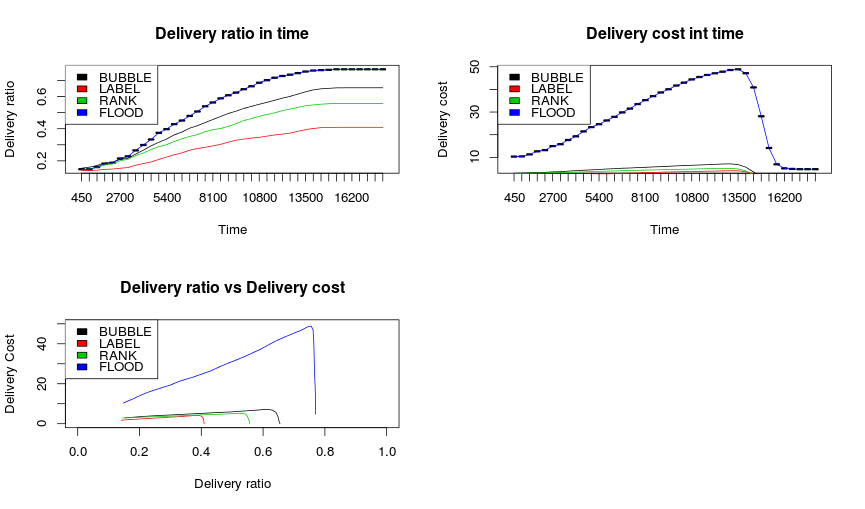
\includegraphics[scale=0.55]{img/run_1_aggregate.pdf}
    		\caption{Experimental session n.1 aggregated data}
    		\label{fig:run_1_aggregate}
\end{figure}
\begin{figure}[h!]
		\centering
    		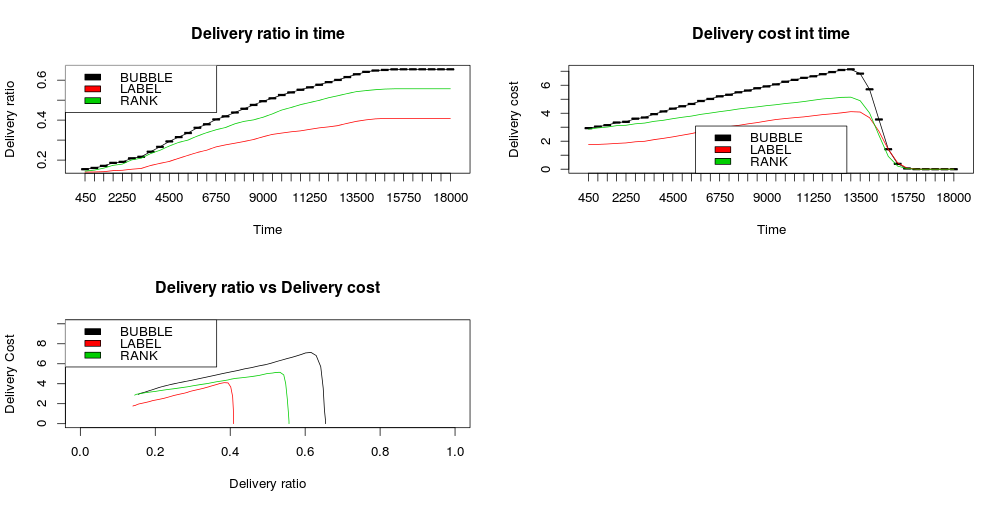
\includegraphics[scale=0.55]{img/run_1_aggregate_noflood.pdf}
    		\caption{Experimental session n.1 aggregated data without flood algorithm}
    		\label{fig:run_1_aggregate_noflood}
\end{figure}
\end{center}
\newpage
% Aggregated data session 2
\begin{figure}[h!]
	\begin{center}
    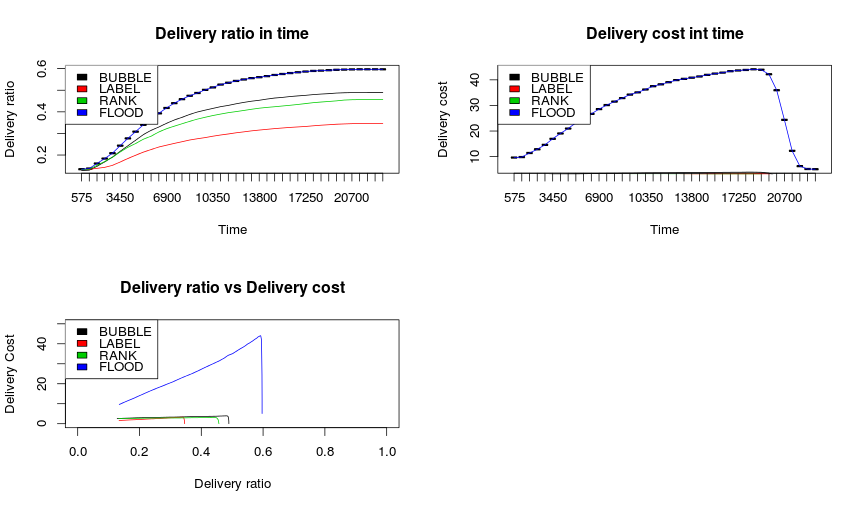
\includegraphics[scale=0.55]{img/run_2_aggregate.pdf}
    \caption{Experimental session n.2 aggregated data}
    \label{fig:run_2_aggregate}
  \end{center}
\end{figure}

\begin{figure}[h!]
	\begin{center}
    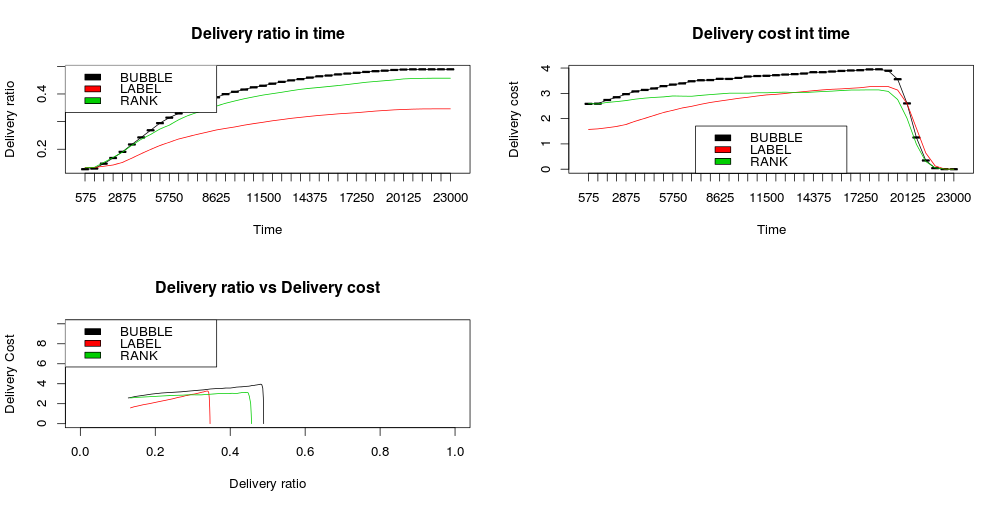
\includegraphics[scale=0.55]{img/run_2_aggregate_noflood.pdf}
    \caption{Experimental session n.2 aggregated data without flood algorithm}
    \label{fig:run_2_aggregate_noflood}
  \end{center}
\end{figure}
\newpage

While in figure ~\ref{fig:run_1_gstats} ~\ref{fig:run_2_gstats} are shown statistics about simulation session 1 and 2 subdivided per algorithm, and in ~\ref{fig:run_1_max_delratio} ~\ref{fig:run_2_max_delratio} are represented the distribution of the delivery ration across the runs.
% Statistics session 1
\begin{figure}[h!]
	\begin{center}
    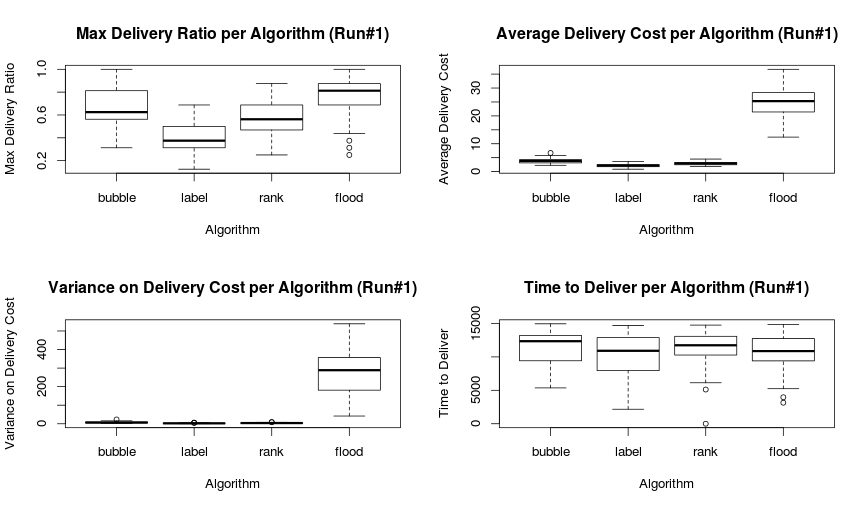
\includegraphics[scale=0.55]{img/run_1_gstats.pdf}
    \caption{Experimental session n.1 statistics}
    \label{fig:run_1_gstats}
  \end{center}
\end{figure}
% Statistics session 2
\begin{figure}[h!]
	\begin{center}
    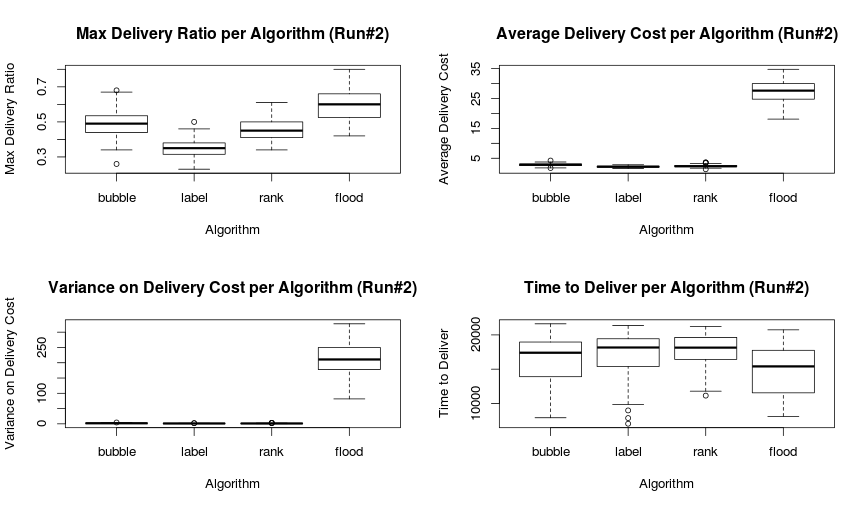
\includegraphics[scale=0.55]{img/run_2_gstats.pdf}
    \caption{Experimental session n.2 statistics}
    \label{fig:run_2_gstats}
  \end{center}
\end{figure}
\newpage
% Del ratio distribution session 1
\begin{figure}[h!]
	\begin{center}
    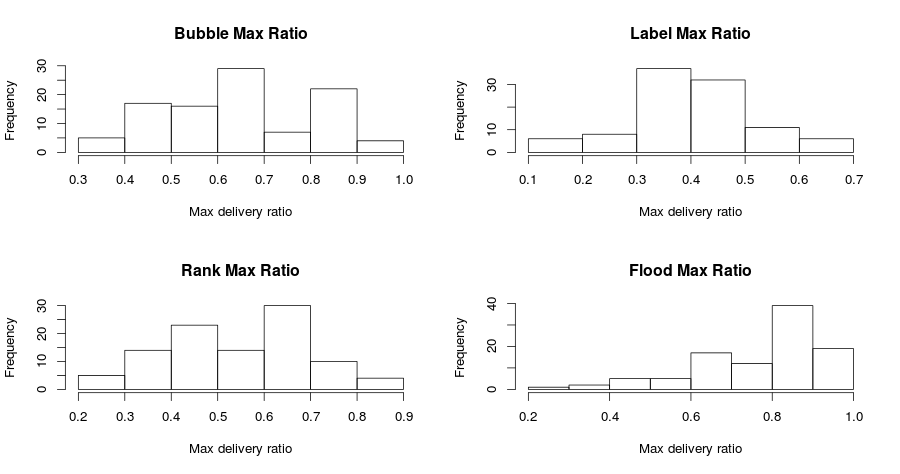
\includegraphics[scale=0.55]{img/run_1_max_delratio.pdf}
    \caption{Experimental session n.1 delivery ratio distribution}
    \label{fig:run_1_max_delratio}
  \end{center}
\end{figure}
% Del ratio distribution session 2
\begin{figure}[h!]
	\begin{center}
    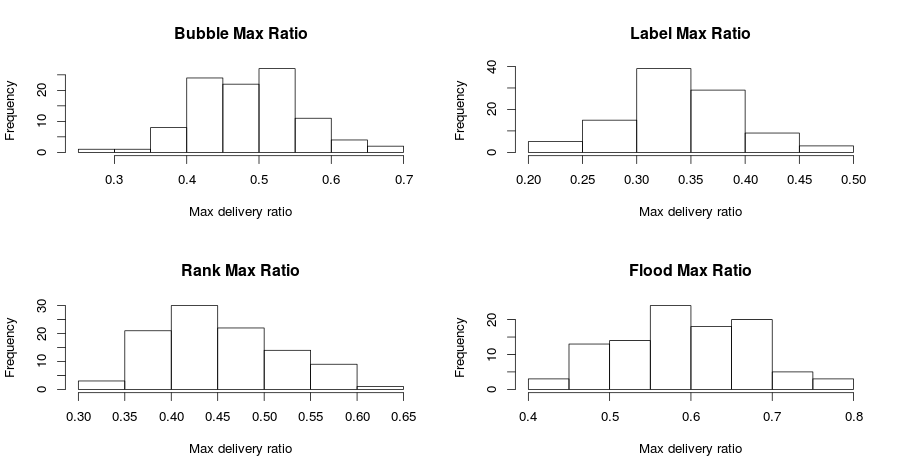
\includegraphics[scale=0.55]{img/run_2_max_delratio.pdf}
    \caption{Experimental session n.2 delivery ratio distribution}
    \label{fig:run_2_max_delratio}
  \end{center}
\end{figure}
\newpage